
\documentclass[12pt]{article}
\usepackage{fullpage,amsmath,amssymb,graphicx}

\usepackage{setspace}
\spacing{1}

\usepackage{textpos}
\usepackage{tikz}
\usepackage{pgf}
\usepackage{amssymb}
\usepackage{enumerate}
\usepackage{xcolor}
\usepackage{graphicx}
\usepackage{subcaption}
\usepackage{tabularx}
\usepackage{colortbl}
\usepackage{multicol}
\usepackage{longtable}
\usepackage{hyperref}
\usepackage{comment}
\usepackage{listings}



\definecolor{encabezado}{rgb}{0.74, 0.83, 0.9}

\begin{document}

\hfill\\
\rule{\textwidth}{1.5pt}

\begin{minipage}[t]{85mm}
  \begin{tabular}{l}
    \textbf{\large Instituto Tecnológico de Costa Rica} \\  
    \textbf{Escuela de Ingeniería Electrónica} \\
    \textbf{Trabajo Final de Graduación} \\
    \textbf{Proyecto:} Método basado en aprendizaje reforzado \\para el control automático de una planta no lineal. \\
    \textbf{Estudiante:} Oscar Andrés Rojas Fonseca \hspace{3cm}\rule{4.5cm}{1.5pt}\\
    I Semestre 2024 \hspace{8.5cm}\textbf{Firma del asesor}
  \end{tabular}
\end{minipage}
\hfill\\
\rule{\textwidth}{1.5pt}


\section*{Bitácora de trabajo}

%\begin{table}[h]
\begin{minipage}[h]{\textwidth}
	\centering
	\begin{tabularx}{\textwidth}{|p{2cm}|X|X|p{2cm}|} 
		\hline
		\rowcolor{encabezado}
		\textbf{Fecha} & 
		\textbf{Actividad} & 
		\textbf{Anotaciones} & 
		\textbf{Horas dedicadas} \\ \hline
		% ***************************************************************
	 	15/04/2024 & 
	 	$\mathbf{1}.$ Redefinición de la conversión del código para valores discretos ($CartPole$) a valores continuos ($Pendulum$). & 
	 	$a)$ El error en $select\_ action()$ se corrigió pero desconfiguró parte de la función $optimize\_ model()$. \newline
	 	$b)$ Corrección del error en $optimize\_ model()$. \newline
	 	$c)$ Persisten los problemas de indexado y proceso. \newline & 
	 	6 horas \\
	 	% ***************************************************************
	 	15/04/2024 & 
	 	$\mathbf{2}.$ Pruebas de entrenamiento del modelo ($Pendulum$). & 
	 	$a)$ Se entrenaron cuatro modelos diferentes a $600$ episodios para comparar el efecto de cuatro propuestas de redes neuronales artificiales (ANN). \newline & 
	 	6 horas \\
		% ***************************************************************
		16/04/2024 & 
	 	$\mathbf{2}.$ Búsqueda de la teoría de los métodos $PPO$ y $actor-critic$ dada la necesidad del manejo del \textit{action space} con valores continuos. &
	 	$a)$ SASASASAS. \newline & 
	 	4 horas \\
	 	% ***************************************************************
	 	17/04/2024 & 
	 	$\mathbf{3}.$ Reunión de seguimiento con el asesor del proyecto. & 
	 	$a)$ Revisión de avance en el código y errores de forma.  \newline
	 	$b)$ Se acordó continuar con el interés en los métodos como $PPO$ como opción para el control.  \newline & 
	 	2 horas \\
		% ***************************************************************
		17/04/2024 & 
	 	$\mathbf{2}.$ Búsqueda de métodos para el manejo de valores continuos en $DQN$. &
	 	$a)$ Aparece el $DDPG$. \newline
	 	$b)$ Opción de discretizar el action space. \newline & 
	 	4 horas \\
	 	% ***************************************************************
		17/04/2024 & 
	 	$\mathbf{2}.$ Prueba de discretización del \textit{action space} del env $Pendulum$. &
	 	$a)$ Se logró adaptar el código del $PendulumDQN$ a una versión discretizada $PendulumDQN_discrete$, depende principalmente de la resolución seleccionada ($n_actions$). \newline
	 	$b)$ Pruebas de entrenamiento de hasta $100$ episodios. \newline & 
	 	4 horas \\
	 	% ***************************************************************
	 	\hline
	\end{tabularx}
\end{minipage}	 	
	 	
	 	% ***************************************************************
\hfill\\
\begin{minipage}[h]{\textwidth}
	\centering
	\begin{tabularx}{\textwidth}{|p{2cm}|X|X|p{2cm}|} 
		\hline		
		
	 	% ***************************************************************
	 	19/04/2024 & 
	 	$\mathbf{4}.$ Corrección de potenciales errores en el código $PendulumDQN$ señalados por asesor. &
	 	$a)$ Replanteo de función de recompensa $calculate\_ reward()$ para evitar salto. \newline
	 	$b)$ Adición de lógica para guardado de $checkpoints$ al entrenamiento y corrección del guardado del modelo. \newline & 
	 	6 horas \\
	 	% ***************************************************************
	 	20/04/2024 & 
	 	$\mathbf{4}.$ Montaje y primera prueba del código \href{https://github.com/ericyangyu/PPO-for-Beginners/tree/master}{$PPO$} para $Pendulum$. &
	 	$a)$ Revisión del error por cambio de versión $Gym$ a $Gymnasium$. \newline
	 	$b)$ Implementación del procesamiento $CUDA$ en el código. \newline & 
	 	6 horas \\
	 	% ***************************************************************
	 	21/04/2024 & 
	 	$\mathbf{4}.$ Prueba de entrenamiento con versión base del $PPO$ para $Pendulum$. &
	 	$a)$ Entrenamiento del modelo con $render("human")$ de $200k$ episodios. Mal desempeño. \newline
	 	$b)$ Entrenamiento del modelo con $render("rgb\_ array")$ de $200M$ de episodios. En proceso. \newline & 
	 	6 horas \\
	 	% ***************************************************************
	 	
	 	\hline
		\multicolumn{3}{|r|}{Total de horas de trabajo:} & 21 horas \\ 
	 	\hline                 
	\end{tabularx}
\end{minipage}
%\end{table}



% *****************************************************************************
% *****************************************************************************
% *****************************************************************************

\section*{Contenidos de actividades}

AAA \cite{DQNCart}.

%\begin{figure}[h]
%	\centering
%	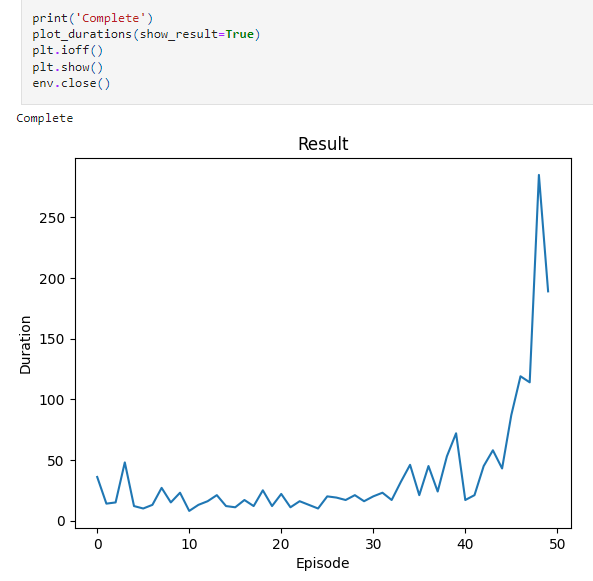
\includegraphics[scale=0.6]{Fig/CapturaCartPole1.png}
%	\caption{Resultado de entrenamiento del modelo para $CartPole$ con $50$ episodios.}
%	\label{fig:Cart1}
%\end{figure}	

\newpage

\section*{Referencias}
\renewcommand\refname{}
\bibliographystyle{IEEEtran}
\bibliography{references}





\end{document}
